% define documentclass
\documentclass[12pt, bibliography=totoc, a4paper, abstractoff, numbers=noenddot]{scrreprt}

% define used packages
\usepackage[left=4.0cm, right=2.0cm, top=3cm, bottom=3cm]{geometry}
\usepackage{bibgerm}
\usepackage[utf8]{inputenc}
\usepackage[T1]{fontenc}
\usepackage{graphicx}
\usepackage[ngerman]{babel}
\usepackage{lmodern}
\usepackage{listings}
\usepackage[numbers]{natbib}
\usepackage{acronym}
\bibliographystyle{alphadin}
\usepackage{float}

\usepackage{lastpage}

% advanced tables
\usepackage{array}

% header and footer
\usepackage{fancyhdr}

% links
\usepackage{url}

% internal links
\usepackage[colorlinks=true ,linkcolor=black,
			anchorcolor=black ,citecolor=black ,filecolor=black,
			menucolor=black ,urlcolor=black]{hyperref}

% mathematical formulas
\usepackage{amsmath, amssymb}

% fancy Diagrams %
\usepackage{tikz}
\usepackage{epstopdf}

% to include images side by side
\usepackage{subfigure}

% for nice bg on title page
\usepackage{eso-pic}
\newcommand\BackgroundPic{%
\put(0,0){%
\parbox[b][\paperheight]{\paperwidth}{%
\vfill
\centering
\includegraphics[width=\paperwidth,height=\paperheight,%
keepaspectratio]{images/Logo_H-BRS_background}%
\vfill
}}}

% define the programming language
\usepackage{listings}
\lstloadlanguages{Java,sh,bash,Haskell,HTML,PHP,XML}
\lstdefinelanguage{console}{
  morekeywords={},
  otherkeywords={warumgehtdasnicht>,\$}
}
\newcommand{\lstsetconsole}
{ \lstset{%language=sh,
        lineskip=-2pt,
        breaklines=true,
        language=console,
        breaklines=true,
        captionpos=b,
        commentstyle=\textit,
        keywordstyle=\bfseries,
        basicstyle=\ttfamily,
        stringstyle=\ttfamily,
        showstringspaces=false,
        frame=single,
        tabsize=2
  }
}
\lstdefinelanguage{scalaconsole}{
  morekeywords={},
  otherkeywords={scala>,\|}
}
\newcommand{\lstsetrepl}
{ \lstset{%language=sh,
        lineskip=-2pt,
        breaklines=true,
        language=scalaconsole,
        breaklines=true,
        commentstyle=\textit,
        keywordstyle=\bfseries,
        basicstyle=\ttfamily,
        stringstyle=\ttfamily,
        showstringspaces=false,
        frame=single,
        tabsize=2
  }
}
\newcommand{\lstsetjava}{
 \lstset{language=Java,
        breaklines=true,
        commentstyle=\textit,
        keywordstyle=\bfseries,
        basicstyle=\ttfamily,
        stringstyle=\ttfamily,
        showstringspaces=false,
        frame=single,
        captionpos=b,
        tabsize=2,
        literate=
        %linewidth=\textwidth,captionpos=b
        %numbers=left, stepnumber=5, numbersep=10pt
 }
}
\lstdefinelanguage{scala}{
  morekeywords={abstract,case,catch,class,def,%
    do,else,extends,false,final,finally,%
    for,forSome,if,implicit,import,lazy,match,mixin,%
    new,null,object,override,package,%
    private,protected,requires,return,sealed,%
    super,this,throw,trait,true,try,%
    type,val,var,while,with,yield},
  otherkeywords={_,:,=,=>,<-,<\%,<:,>:,\#,@},
  sensitive=true,
  morecomment=[l]{//},
  morecomment=[n]{/*}{*/},
  morestring=[b]",
  morestring=[b]',
  morestring=[b]"""
}
\newcommand{\lstsetscala}{
 \lstset{language=scala,
        breaklines=true,
        commentstyle=\textit,
        keywordstyle=\bfseries,
        basicstyle=\ttfamily,
        stringstyle=\ttfamily,
        showstringspaces=false,
        frame=single,
        tabsize=2
        %%linewidth=\textwidth,captionpos=b
        %numbers=left, stepnumber=5, numbersep=10pt
 }
}
\newcommand{\lstsethtml}{
 \lstset{language=HTML,
        breaklines=true,
        commentstyle=\textit,
        keywordstyle=\bfseries,
        basicstyle=\ttfamily,
        stringstyle=\ttfamily,
        showstringspaces=false,
        frame=single,
        tabsize=2
        %%linewidth=\textwidth,captionpos=b
        %numbers=left, stepnumber=5, numbersep=10pt
 }
}
\newcommand{\lstsetphp}{
 \lstset{language=PHP,
        breaklines=true,
        commentstyle=\textit,
        keywordstyle=\bfseries,
        basicstyle=\ttfamily,
        stringstyle=\ttfamily,
        showstringspaces=false,
        frame=single,
        tabsize=2
        %%linewidth=\textwidth,captionpos=b
        %numbers=left, stepnumber=5, numbersep=10pt
 }
}
\lstnewenvironment{code}
    {\lstset{}%
      \csname lst@SetFirstLabel\endcsname}
    {\csname lst@SaveFirstLabel\endcsname}
\newcommand{\lstsethaskell}{
    \lstset{
      language=Haskell,
      commentstyle=\textit,
      keywordstyle=\bfseries,
      basicstyle=\ttfamily,
      stringstyle=\ttfamily,
      showstringspaces=false,
      frame=single,
      flexiblecolumns=false,
      basewidth={0.5em,0.45em},
      literate={+}{{$+$}}1 {/}{{$/$}}1 {*}{{$*$}}1 {=}{{$=$}}1
               {==}{{$==$}}2 %{!=}{{$\not\equiv$}}2
               {>}{{$>$}}1 {<}{{$<$}}1 {\\}{{$\lambda$}}1
               {\\\\}{{\char`\\\char`\\}}1
               {->}{{$\rightarrow$} }2 {>=}{{$\geq$}}2 {<-}{{$\leftarrow$}}2
               {<=}{{$\leq$}}2 {=>}{{$\Rightarrow$} }2
               {\ .}{{$\circ$}}2 {\ .\ }{{$\circ$}}2 {(.)}{({$\circ$})}2
               {>>}{{>>}}2 {>>=}{{>>=}}2
               {|}{{$\mid$}}1
    }
}
\lstdefinelanguage{JavaScript}{
  keywords={typeof, new, true, false, catch,%
    function, return, null, catch, switch, var,%
    if, in, while, do, else, case, break},
  ndkeywords={class, export, boolean, throw, implements, import, this},
  sensitive=false,
  comment=[l]{//},
  morecomment=[s]{/*}{*/},
  morestring=[b]',
  morestring=[b]"
}
\newcommand{\lstsetjavascript}{
  \lstset{
		language=JavaScript,
		breaklines=true,
		commentstyle=\textit,
		basicstyle=\ttfamily,
		keywordstyle=\bfseries,
		stringstyle=\ttfamily,
		showstringspaces=false,
		frame=single,
		tabsize=2
  }
}
\newcommand{\lstsetxml}{
 \lstset{language=XML,
        breaklines=true,
        commentstyle=\sffamily,
        keywordstyle=\bfseries,
        basicstyle=\sffamily,
        showstringspaces=false,
        stringstyle=\ttfamily,
        frame=single,
        tabsize=2,
        literate=
        %linewidth=\textwidth,captionpos=b
        %numbers=left, stepnumber=5, numbersep=10pt
 }
}
\lstdefinelanguage{CSharp}{
 morekeywords = {abstract,event,new,struct,as,explicit,%
    null,switch,base,extern,object,this,bool,false,%
    operator,throw,break,finally,out,true,byte,fixed,%
    override,try,case,float,params,typeof,catch,for,%
    private,uint,char,foreach,protected,ulong,checked,%
    goto,public,unchecked,class,if,readonly,unsafe,%
    const,implicit,ref,ushort,continue,in,return,using,%
    decimal,int,sbyte,virtual,default,interface,sealed,%
    volatile,delegate,internal,short,void,do,is,sizeof,%
    while,double,lock,stackalloc,else,long,static,%
    enum,namespace,string,partial},
  morecomment = [l]{//},
  morecomment = [l]{///},
  morecomment = [s]{/*}{*/},
  morestring=[b]",
  sensitive = true
}
\newcommand{\lstsetcsharp}{
 \lstset{language=csharp,
        breaklines=true,
        commentstyle=\sffamily,
        basicstyle=\sffamily,
        keywordstyle=\bfseries,
        stringstyle=\ttfamily,
        showstringspaces=false,
        frame=single,
        tabsize=2
        %%linewidth=\textwidth,captionpos=b
        %numbers=left, stepnumber=5, numbersep=10pt
 }
}
\lstdefinelanguage{FSharp}{
  morekeywords={abstract,and,as,assert,base,begin,%
    class,default,delegate,do,done,downcast,downto,%
    elif,else,end,exception,extern,false,finally,for,fun,%
    function,if,in,inherit,inline,interface,internal,lazy,%
    let,match,member,module,mutable,namespace,%
    new,not,null,of,open,or,override,private,public,rec,%
    return,static,struct,then,to,true,try,type,upcast,use,%
    val,void,when,while,with,yield,asr,land,lor,lsl,lsr,lxor,%
    mod,sig,atomic,break,checked,component,const,%
    constraint,constructor,continue,eager,event,external,%
    fixed,functor,global,include,method,mixin,object,%
    parallel,process,protected,pure,sealed,tailcall,trait,virtual,volatile},     
  sensitive=false,
  morecomment=[l][\color{greencomments}]{///},
  morecomment=[l][\color{greencomments}]{//},
  morecomment=[s][\color{greencomments}]{{(*}{*)}},
  morestring=[b]"
}
\newcommand{\lstsetfsharp}{
 \lstset{language=fsharp,
        breaklines=true,
        commentstyle=\sffamily,
        basicstyle=\sffamily,
        keywordstyle=\bfseries,
        stringstyle=\ttfamily,
        showstringspaces=false,
        frame=single,
        tabsize=2
        %%linewidth=\textwidth,captionpos=b
        %numbers=left, stepnumber=5, numbersep=10pt
 }
}

%set default pagestyle
\pagestyle{empty}

\setlength{\parindent}{0pt}
\setlength{\parskip}{12pt}

% #####
% #
% # START config area
% #
% #####

\newcommand{\HEADER}[0]{H-BRS, WS 2018}
\newcommand{\PAGENUMBERS}[0]{\pagemark}
\newcommand{\DATE}[0]{\today}

\newcommand{\AUTHOR}[0]{Ben Kirsche}
\newcommand{\MATNR}[0]{123456}
\newcommand{\STREET}[0]{Humperdinckstraße 20}
\newcommand{\ZIP}[0]{53721}
\newcommand{\TOWN}[0]{Siegburg}

\newcommand{\REFERENT}[0]{Prof. Dr. Harm Knolle}
\newcommand{\KOREFERENT}[0]{}

\newcommand{\TITLE}[0]{Anwendungsszenarien für Graphdatenbanken}
\newcommand{\COURSE}[0]{Studiengang Informatik}
\newcommand{\TYPE}[0]{Projektarbeit}
\newcommand{\COMPLETION}[0]{Master of Science}

% #####
% #
% # END config area
% #
% #####

% Hurenkinder und Schusterjungenregelung
\clubpenalty=100000
\widowpenalty=100000
\displaywidowpenalty=100000

% starting the document
\begin{document}

% set pagenumbering to roman(I II III IV)
\pagenumbering{Roman}
% input the title
% #####
% #
% # This is the titlelayout from Prof. Dr. Harm Knolle 
% # (Hochschule Bonn-Rhein-Sieg)
% #  
% #####

% #####
% #
% # Default layout
% #
% #####

%\AddToShipoutPicture*{\BackgroundPic}

\begin{titlepage}
  \begin{center}
  	
\includegraphics[scale=1]{./images/LogoH-BRS.jpg}
  \end{center}
  \vspace{40pt}
  \sffamily
  \begin{tabular}{|l>{\raggedright\hspace{0pt}\arraybackslash}p{15cm}}
    & \\
    & \large\textbf{\TYPE}\\[\baselineskip]
    & \huge\textbf{\TITLE}\\[\baselineskip]
    & - \COURSE\ -\\
    & \\
  \end{tabular}
  \vfill
  \begin{tabular}{ll@{}}
    & Fachbereich Informatik\\[\baselineskip]
    &   Referent: \REFERENT\\[\baselineskip]
    & \\[\baselineskip]
    & eingereicht von:\\[\baselineskip]
    & \AUTHOR\\[\baselineskip]
    & Matr.-Nr. \MATNR\\[\baselineskip]
    & \STREET\\[\baselineskip]
    & \ZIP \ \TOWN\\[\baselineskip]
    & \\[\baselineskip]
    & Sankt Augustin, den \DATE\\[\baselineskip]
  \end{tabular}
\end{titlepage}


\begin{abstract}
\section*{Zusammenfassung}\markboth{Zusammenfassung}{}
Im Rahmen der Master-Veranstaltung „Schemalose Datenbanken“ soll eine Ausarbeitung zum Thema  „Graphdatenbanken: Anwendungsszenarien und Implementierungen mit MariaDB-OQGRAPH“ erarbeitet werden. Zu diesem Zweck haben sich die drei Autoren zu der Arbeitsgruppe 1 zusammengeschlossen.

Die Ausarbeitung lässt sich in zwei grundsätzliche Teile gliedern. Der erste Teil ist von theoretischer Natur und betrachtet Anwendungsszenarien von Graphdatenbanken. Anhand einer breiten Auswahl von Business Cases soll nicht nur der Mehrwert von Graphdatenbanken in den entsprechenden Szenarien festgehalten, sondern auch eine Abgrenzung zu konkurrierenden, relationalen Ansätzen erörtert werden.

Folgende Szenarien werden vorgestellt:
\begin{itemize}
	\item Text-Mining, Natural Language Processing
	\item Soziale Netze
	\item Betrugserkennung
	\item Empfehlungs-Engine
	\item Verkehrsnetze
	\item Stammdatenmanagement
\end{itemize}

Der zweite Teil dieser Ausarbeitung wird eine praktische Umsetzung mittels MariaDB OQGRAPH \cite{oqgraph} sein. Zuvor wird noch das System, insbesondere seine Eigenheit, vorgestellt und die Installation auf dem Hochschulrechner dokumentiert.

Dieser Teil besteht aus zwei Anwendungen, die jeweils andere Anforderungen an eine Graphdatenbank stellen. Die erste Anwendung ist eine OLTP System in der Form eines Gästebuchs. Im Fokus steht dabei vor allem die Aspekte der Modellierung, dafür wird das eigentliche Modell in QOGRAP erstellt. Im Zuge dessen werden die Unterschiede, insbesondere die Vorteile, im Vergleich zu einem relationalem Ansatz erarbeitet. Des weiteren werden diverse Use Cases implementiert, die über ein eigens dafür entworfenes, simples Frontend gesteuert werden können.

Die zweite Anwendung ist ein einfaches soziales Netz, mit Nutzern und Kontakten. Hierbei handelt es sich um eine OLAP-System. Im Gegensatz zu der vorherigen Anwendung, wird hier die Modellierung nicht weiter beachtet. Der Fokus liegt stattdessen auf der Performance der Graphdatenbank. Betrachtet werden Projektion und Selektion über unterschiedliche Zugriffsmöglichkeiten, sowie Traversierung und Aggregation der Datensätze. Anhand diverser Metriken werden die Messungen evaluiert.
\nocite{*}
\end{abstract}


% load the preamble
%% \renewcommand\abstractname{Danksagung}
\begin{abstract}
\section*{Vorwort}\markboth{Vorwort}{}
  \addcontentsline{toc}{chapter}{Vorwort}
\end{abstract}

% loads the fancy pagestyle for register part
% set the pagestyle to fancy
\pagestyle{fancy}

\fancyhf{}% clear all fields
  % define the header
  \fancyhead[L]{\leftmark}% left header
  \fancyhead[R]{\HEADER}% right header
  \renewcommand{\headrulewidth}{0.4pt}% top line

  % define the footer
  \fancyfoot[L]{\AUTHOR}% left footer
  \fancyfoot[R]{\pagemark}% right footer
  \renewcommand{\footrulewidth}{0.6pt}% bottom line

  % redefine the chaptermark to have '1. Chaptername' and not 'CHAPTER 1.
  % CHAPTERNAME'
  \renewcommand{\chaptermark}[1]{\markboth{\thechapter.\ #1}{}}

% override the plain style
\fancypagestyle{plain}{%
\fancyhf{}% clear all fields
  % define the header
  \renewcommand{\headrulewidth}{0.0pt}% top line

  % define the footer
  \fancyfoot[L]{\AUTHOR}% left footer
  \fancyfoot[R]{\pagemark}% right footer
  \renewcommand{\footrulewidth}{0.6pt}% bottom line
}


% create the registers
\tableofcontents\newpage

% set pagenumbering to arabic(1 2 3 4)
\pagenumbering{arabic}
% loads the fancy pagestyle for main part
% set the pagestyle to fancy
\pagestyle{fancy}

\fancyhf{}% clear all fields
  % define the header
  \fancyhead[L]{\leftmark}% left header
  \fancyhead[R]{\HEADER}% right header
  \renewcommand{\headrulewidth}{0.4pt}% top line

  % define the footer
  \fancyfoot[L]{\AUTHOR}% left footer
  \fancyfoot[R]{\PAGENUMBERS}% right footer
  \renewcommand{\footrulewidth}{0.6pt}% bottom line

  % redefine the chaptermark to have '1. Chaptername' and not 'CHAPTER 1.
  % CHAPTERNAME'
  \renewcommand{\chaptermark}[1]{\markboth{\thechapter.\ #1}{}}

% override the plain style
\fancypagestyle{plain}{%
\fancyhf{}% clear all fields
  % define the header
  \renewcommand{\headrulewidth}{0pt}% top line

  % define the footer
  \fancyfoot[L]{\AUTHOR}% left footer
  \fancyfoot[R]{\PAGENUMBERS}% right footer
  \renewcommand{\footrulewidth}{0.6pt}% bottom line
}


% #####
% # load the chapter from the files
% #####
\chapter{Anwendungsszenarien}
\section{Text-Mining, Natural Language Processing}
\section{Soziale Netze}
Unter dem Begriff Sozialem Netz versteht man eine Menge an Teilnehmern, häufig sind dies natürliche Personen, und verschiedenen Arten an Relationen zwischen diesen. Das durch die Beziehungen gebildete Netz lässt sich problemlos als Graph darstellen, indem die Teilnehmer als Knoten des Graphen dargestellt und die Beziehungen auf die Kanten abgebildet werden.

\begin{figure}
	\caption{Auschnitt aus Facebooks Socail-Graph: Checkin \cite{facebookTao}}
	\label{fig:fbCheckin}
	\centering
	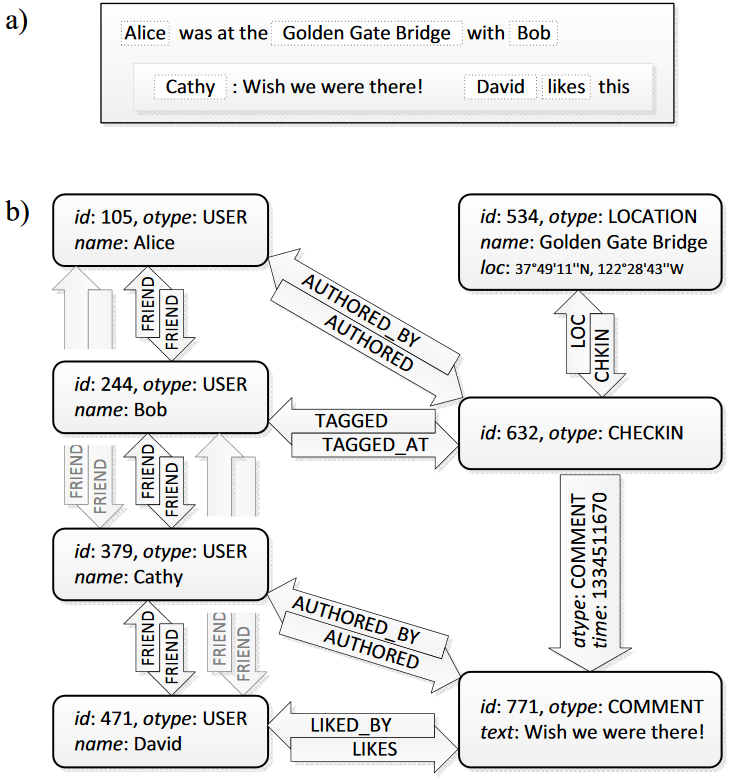
\includegraphics[width=0.7\textwidth]{images/facebook_checkin.png}
\end{figure}

Abbildung~\ref{fig:fbCheckin} zeigt beispielhaft wie ein Teil des Sozialen Netzes von Facebook aussieht. Anhand solcher Einträge wird für jeden einzelnen Nutzer eine personalisierte Startseite in Echtzeit erzeugt, dementsprechend wichtig ist ein performanter Datenzugriff. Um den Anforderungen gerecht zu werden hat Facebook eine eigene Graph-ähnliche API namens TAO entwickelt, welche den Datenbankzugriff effizient steuert. TAO stellt minimale Create/Update/Delete-Kommandos für Knoten und Kanten bereit. Der Großteil der Datenbankzugriffe ist allerdings lesend, folgende Querys sind möglich \cite{facebookTao}:
\begin{itemize}
	\item Alle Assoziation eines Typs zu einem Knoten
	\item Anzahl der Assoziationen eines Typs an einem Knoten
	\item Alle Nachbarn bis zur Tiefe n über eine bestimmte Assoziation
\end{itemize}
Dies ist ausreichend um mittels Verfahren wie Zentralitätsberechnung, Dichte und Cliquenanalyse für den Nutzer relevante Beiträge zu bestimmen \cite{sozialeNetzwerkanalyse}.


\section{Betrugserkennung}
Graph Datenbanken werden in e-commerce benutzt um die Betrug zu vermeiden. In Graph Datenbanken ist es möglich das Suchen der verdächtigen Pattern einzustellen - die entsprechenden Prüfungen, die mit den verschiedenen Triggern verbunden sind. Diese Triggern lassen sich die Probleme identifizieren, bevor als der ernschafte Schaden getroffen wird. Triggern können aus die nächste Ereignissen besteht werden: Einloggen in System, Registrierung einer neuen Bankkarte oder Bestellung der Waren.
\begin{figure}
	\caption{Transaktionsserie}
	\label{fig:Trs}
	\centering
	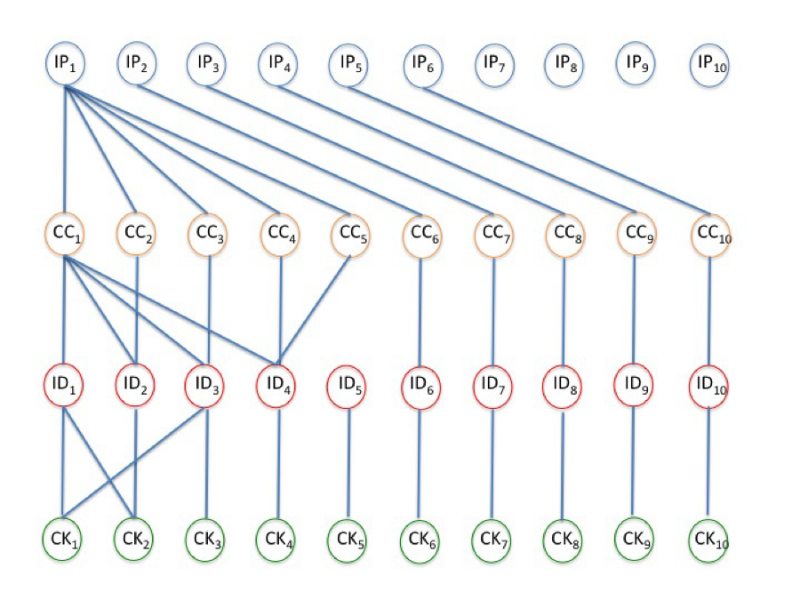
\includegraphics[width=0.7\textwidth]{images/Betrugserkennung.png}
\end{figure}

Auf der Abbildung~\ref{fig:Trs} sind die Transaktionsserien von den verschiedenen IP Adressen gezeigt. (IP(x) - IP Adresse, CC(x) - die Nummer der Kreditkarte, ID(x) - der Identifikator vom Nutzer, CK(x) - das Cookie, das im Systeme enthält). In diesem Beispiel ist es vermutlich, dass IP(1) von den Betrugen benutzt wird, denn vom IP(1) sind viele Transaktionen mit den unterschidliechen Kreditkarten durchgeführt, und eine Karte wurde von mehreren Nutzer benutzt, einige der auch mehr als eine Cookie besitzen. 
Graph Datenbanken sind die idealerweise Lösung der Bedrohungsentdeckung, die mit dem Finanzsicherheit in Netz verbunden sind, denn die Aktivität der Angreifern entspricht in jedem Fall zu einigen Pattern, und wenn sie rechtzeitig erkannt werden, können die möglichen Schaden minimiert werden.

\section{Empfehlungs-Engine}
Die Empfehlungsalgorithmen stellen die Verbindung zwischen den Leuten und den Dingen ein (die Waren, Dienstleistungen, Media-content) - alles, was relevant in diesem Bereich ist, wo diese Empfehlungsalgorithmen verwendet werden. Die Beziehungen werden basiert auf Benutzerverhalten. (Einkaufen, Bewertung, usw)
Die Effektivität der Empfehlungen hängt von dem Verstehen der Beziehungen zwischen Dingen ab und auch die Verbindung -qualität und -stärke. Diese Struktur ist am besten in Form von den attributierten Graphen vorgestellt. Die Anfragen in den Graphen sind meistens lokal, weil ihr Startpunkte ein oder einige identifizierte Objekte ist, und die weitere Suche ist in der Nähe von dieser Objekten durcgefürt.
Eine der ersten Empfehlungsalgorithmen war das System des Internet-Handels Amazon. Ein weiterentwickeltes Empfehlungsalgorithmus wurde von Google hergestellt. In diesem System war erstmal das Sammlungsverfahren der Nutzersinformationen verwendet worden, das cookies während der Besuchung der Suchmaschinen-Website benutzt wird und aufgrund der Suchensergebnisse wurde das Profil für jeden Nutzer aufgebaut.

\section{Verkehrsnetze}
\section{Stammdatenmanagement}
Stammdaten heißen die Daten, die kritisch wichtig für die Geschäftstransaktionen. Die Basisdaten enthält die Daten über die Benutzer, Einkäuferen, Produkten, Lieferanten, Abteilungen, Webseiten, usw. In den größen Organisationen sind solche Daten stark verteilt und heterogen nach den Formaten, Qualität und Zugangsmitteln. Das Stammdatenmanagement enthält die Identifizierung, Löschung, Speicherung und entsprechend Datenverwaltung. Das Stammdatenmanagement soll an der Veränderung der Oraganisationsstruktur, Verschmelzung von den Organisationen, Änderung der Geschäftsregeln usw. angepasst werden. Graph Datenbanken werden gut für die Modelirung, Speicherung, und Anfragen zu den Basismetadaten und Stammdatenmodellen gepasst werden. 


\subsection{Installation}\label{Installation}
In diesem Kapitel wird die Installation und Konfiguration des DBS MaraiDB, sowie des Plugins QOGRAPH auf einem Ubuntu Rechner beschrieben.  
QOGRAPH wird als Plugin in einem eigenständigem Softwarepaket verteilt. Es ist nicht zwingend nötig den MariaDB-Server explizit zu installieren, dieser ist als Abhängigkeit definiert und wird automatisch mit installiert, wenn keine gültige Installation gefunden wird. Alle benötigten Pakete können mittels apt-get installiert werden.
\begin{lstlisting}
sudo apt-get install mariadb-plugin-oqgraph
\end{lstlisting}
Danach muss das Plugin noch installiert werden. Dafür in die DBMS-Konsole \texttt{mysql} wechseln und folgendes Kommando eingeben. Die Installation ist damit abgeschlossen.
\begin{lstlisting}
INSTALL SONAME 'ha_oqgraph';
\end{lstlisting}

Dabei ist zu beachten, dass MaraiDB das User-Directory von Unix nutzt. Dementsprechend kann nur mit root Rechten in die \texttt{mysql} Konsole  gewechselt werden. Es ist also nötig \texttt{sudo} zu verwenden. Damit auch normale User die Datenbank administrieren können, muss das \texttt{unix\_socket} Plugin deaktiviert werden.

\subsection{Visitenkarte}
\begin{enumerate}
	\item Allgemein
	\begin{enumerate}
		\item Name: MariaDB
		\item Modell: Storage Engines OQGRAPH
		\item Version: MariaDB 10.3.11, OQGRAPH 3.0
		\item Historie: MariaDB enstanden als Abspaltung (Fork) von MySQL, OQGRAPH als Plugin von MariaDB
		\item Hersteller: MariaDB Corporation, MariaDB Foundation
		\item Lizenz: GNU
		\item Quellen: https://mariadb.com/kb/en/library/documentation/, 
		https://dev.mysql.com/doc/internals/en/client-server-protocol.html
	\end{enumerate}
	\item Besonderheiten
	\begin{enumerate}
		\item Vergleichbare Systeme: MySQL
		\item Alleinstellungsmerkmale: OQGRAPH Grapherweiterung auf SQL Basis
	\end{enumerate}
	\item Architektur
	\begin{enumerate}
		\item Programmiersprache (des Systems): C, C++, Perl, Bash
		\item Systemarchitektur: InnoDB, Aria, OQGRAPH
		\item Betriebsart: Multi-User, Standalone, Cluster
		\item Protokoll der Schnittstelle: MySQL-Protocol
		\item API: SQL
	\end{enumerate}
	\item Datenmodell
	\begin{enumerate}
		\item Standardsprache: SQL
		\item Objektbegriff: Tabellen, Spalten, Zeilen, Attribute
		\item Sichten: Views
		\item Datentypen: Numeric, String, Date (in diversen Ausprägungen)
		\item Externe Dateien: BLOB (MEDIUMBLOB, LONGBLOB), TEXT (MEDIUMTEXT, LONGTEXT), JSON
		\item Schlüssel: Primär und Fremdschlüssel
		\item Semantisch unterschiedliche Beziehungen: Assoziation, Generalisierung, Spezifizierung
		\item Sonstige Constraints: Not Null, Check
	\end{enumerate}
	\item Indexe
	\begin{enumerate}
		\item Sekundärindexe: Plain Indexe, Full-Text Indexe
		\item Historische Daten: Transaktionsverwaltung, Logs
		\item Gespeicherte Prozeduren: SQL-Procedures
		\item Triggermechanismen: SQL-Trigger
		\item Versionierung: SYSTEM VERSIONING
	\end{enumerate}
	\item Anfragemethode
	\begin{enumerate}
		\item Kommunikation, Protokoll: MySQL-Protocol (TCP/IP)
		\item CRUD-Operationen: SQL (CREATE, INSERT, SELECT, UPDATE, ALTER, DELETE)
		\item Ad-hoc-Anfragen: Innerhalb spezieller Datenbank-Engines möglich (Casandra, ColumnStore)
		\item Kopplungstechniken: JOIN, UNION
		\item Map/Reduce: Nicht vorhanden
	\end{enumerate}
	\item Horizontale Skalierbarkeit
	\begin{enumerate}
		\item Konfiguration: Datenbank-Engine MaxScale
		\item Sharding: Spider, CONNECT oder Galera
		\item Replikation: GTID (Global Transaction Identifier), Master-Slave-Replikation
	\end{enumerate}
	\item Konsistenz
	\begin{enumerate}
		\item ACID: Erfüllt
		\item Transaktionen: SQL-Standard-Transactions
		\item Nebenläufigkeit (Synchronisation): Vorhanden
		\item Dauerhaftigkeit: Ja
		\item Konfliktbehandlung Replikation: Master-Slave-Replikation, Multi-Soruce-Replication
	\end{enumerate}
	\item Administration
	\begin{enumerate}
		\item Werkzeuge: PHPmyAdmin
		\item Massendatenimport: Load-Data-Infile, CONNECT-Engine
		\item Datensicherheit: Save-Data-Infile, MYSQL-Dump (Logisches Backup), MYSQl-Hotcopy (physikalisches Backup)
		\item Recovery: Engines XtraDB/InnoDB Recovery-Mode
		\item Komprimierung: Je nach Storage Engine
		\item Authentifizierung: In MariaDB integriert, Plugins: ed25519, GSSAPI, NamedPipe, PAM
		\item Mandantenfähigkeit: User und Rechtekonzept, getrennte Datenbanken
	\end{enumerate}
\end{enumerate}

\subsection{Grundlegende Funktionsweise des Systems}\label{chp:funktionsweise}
OQGRAPH ist ein Plugin, welches auf das normale relationale System von MariaDB aufbaut. Eine Graphdatenbank besteht prinzipiell lediglich aus zwei Tabellen. Eine Backing-Tabelle welche die Graphdaten in der Form von Kanten enthält und eine API-Tabelle auf die nur lesend zugegriffen werden kann. Diese zwei Tabellen werden im folgenden genauer beschrieben.

Die Backing-Tabelle ist eine normale relationale SQL Tabelle. Konkrete Anforderungen an diese bestehen nicht. Allerdings ist zu beachten das die API-Tabelle Daten aus Backing-Tabelle ließt und entsprechend gemappt werden muss. Damit dies gelingt muss die Tabelle jeweils eine \emph{not null numeric} Spalte für den Start- und Endknoten einer Kante bereitstellen. Es kann auch ein Kantengewicht gespeichert werden, OQGRAPH erwartet einen \emph{double} Wert. Darüber hinaus kann die Backing-Tabelle weitere beliebige Attribute enthalten. Es empfiehlt sich aber einen zusammengesetzten Primärschlüssel auf den beiden Kantenknoten zu definieren. Des Weiteren sorgt ein zusätzlicher Index auf dem Endknoten für optimale Performance bei den von OQGRAPH bereitgestellten Graphalgorithmen. Eine beispielhafte Implementierung des Schemas ist im Anhang \ref{schemaBacking} zu finden.

Die Api-Tabelle ist aus technischer Sicht ebenfalls nur eine SQL-Tabelle, ihre Aufgabe ist aber die Kapselung der datenhaltende Backing-Tabelle und das bereitstellen diverser Graphalgorithmen. Das Schema dieser Tabelle ist komplett vorgegeben und muss so übernommen werden, eine entsprechende Vorlage ist Anhang \ref{schemaApi} zu finden. Auf dieser Tabelle können mittels SQL-Syntax Graphalgorithmen durchgeführt werden. Die geschieht über ein Select auf der API-Tabelle, über die Where-Klausel können Argumente an die Algorithmen übergeben werden. Das Latch Attribut bestimmt den konkreten Algorithmus, \emph{origid} und \emph{destid} sind die Start und Endpunkte. In der folgenden Tabelle sind alle von OQGRAPH bereitgestellten Operationen aufgelistet.

\begin{tabularx}{\textwidth}{l l X}
	\textbf{Latch Wert }    & \textbf{Where-Klausel}  & \textbf{Graphoperation} \\
	\hline
	(empty string) & origid         & List all first hop vertices from origid in linkid column. \\
	dijkstras      & origid, destid & Find shortest path using Dijkstras algorithm between origid and destid, with traversed vertex ids in linkid column. \\
	dijkstras      & origid         & Find all vertices reachable from origid, listed in linkid column, and report sum of weights of vertices on path to given vertex in weight. \\
	dijkstras      & destid         & Find all vertices from which a path can be found to destid, listed in linkid column, and report sum of weights of vertices on path to given vertex in weight. \\
	breadth\_first & origid         & List vertices reachable from origid in linkid column. \\
	breadth\_first & destid         & List vertices from which a path can be found to destid in linkid column. \\
	breadth\_first & origid, destid & Find shortest path between origid and destid, report in linkid column. \\
	leaves         & origid         & List vertices reachable from origid, that only have incoming edges. \\
	leaves         & destid         & List vertices from which a path can be found to destid, that only have outgoing edges.
\end{tabularx}



\newpage

% loads the fancy pagestyle for register part
% set the pagestyle to fancy
\pagestyle{fancy}

\fancyhf{}% clear all fields
  % define the header
  \fancyhead[L]{\leftmark}% left header
  \fancyhead[R]{\HEADER}% right header
  \renewcommand{\headrulewidth}{0.4pt}% top line

  % define the footer
  \fancyfoot[L]{\AUTHOR}% left footer
  \fancyfoot[R]{\pagemark}% right footer
  \renewcommand{\footrulewidth}{0.6pt}% bottom line

  % redefine the chaptermark to have '1. Chaptername' and not 'CHAPTER 1.
  % CHAPTERNAME'
  \renewcommand{\chaptermark}[1]{\markboth{\thechapter.\ #1}{}}

% override the plain style
\fancypagestyle{plain}{%
\fancyhf{}% clear all fields
  % define the header
  \renewcommand{\headrulewidth}{0.0pt}% top line

  % define the footer
  \fancyfoot[L]{\AUTHOR}% left footer
  \fancyfoot[R]{\pagemark}% right footer
  \renewcommand{\footrulewidth}{0.6pt}% bottom line
}


% #####
% # load the appendix from the files
% #####
%\appendix
\chapter{Anhang}
\section{Schema für die OQGRAPH Backing-Tabelle}\label{schemaBacking}
\begin{lstlisting}
CREATE TABLE oq2_backing (
  origid INT UNSIGNED NOT NULL, 
  destid INT UNSIGNED NOT NULL, 
  weight DOUBLE NOT NULL, 
  PRIMARY KEY (origid, destid), 
  KEY (destid)
);	
\end{lstlisting}
\section{Schema für die OQGRAPH API-Tabelle}\label{schemaApi}
\begin{lstlisting}
CREATE TABLE oq_graph
ENGINE=OQGRAPH 
data_table='oq_backing' 
origid='origid'
destid='destid' 
weight='weight';
\end{lstlisting}
Für MariaDB Versionen älter als 10.1.2 müssen die Attribute manuell spezifiziert werden.
\begin{lstlisting}
CREATE TABLE oq_graph (
  latch VARCHAR(32) NULL,
  origid BIGINT UNSIGNED NULL,
  destid BIGINT UNSIGNED NULL,
  weight DOUBLE NULL,
  seq BIGINT UNSIGNED NULL,
  linkid BIGINT UNSIGNED NULL,
  KEY (latch, origid, destid) USING HASH,
  KEY (latch, destid, origid) USING HASH
) ENGINE=OQGRAPH 
data_table='oq_backing' 
origid='origid' 
destid='destid' 
weight='weight';	
\end{lstlisting}
\section{Installationsscript der OLTP Anwendung}
\lstset{
	columns=fullflexible,
	breaklines=true,
	postbreak=\mbox{\textcolor{red}{$\hookrightarrow$}\space},
}
%\lstinputlisting[language=SQL]{appendix/oltp_create.log}
\section{Messergebnisse des OLAP Systems}
\begin{tabularx}{\textwidth}{X X X X X X}
	\textbf{Test Case}    & \textbf{Facebook}  & \textbf{Wikipedia} & \textbf{Epinions} & \textbf{Youtube} & \textbf{LiveJournal} \\
	\hline
	Selektion PK &	39&	35&	35&	48&	38\\
	PK (Vollständig)&	45&	40&	34&	49&	39\\
	NPK&	1198&	1631&	2762&	34353&	53051\\
	indexierter NPK&	151&	339&	61&	148&	160\\
	Anz. Nutzer&	1180&	2438&	10279&	313073&	1080732\\
	Anz. Beziehungen&	24333&	28018&	46188&	819052&	9255936\\
	AVG Alter&	3226&	4564&	18562&	508547&	1904271\\
	AVG Beziehung&	37821&	47658&	85494&	1444649&	16644672\\
\end{tabularx}

\begin{tabularx}{\textwidth}{X X X X X X X}
	\textbf{Test Case} & \textbf{OQ GRAPH Tab.}    & \textbf{Tiefe=1}  & \textbf{Tiefe=2} & \textbf{Tiefe=3} & \textbf{Tiefe=4} & \textbf{Tiefe=5} \\
	\hline
	Facebook&	1499107&	132& 118& 163&	167& 164\\
	Facebook Business&	281034&	162&	152&	152& 151&	154\\
	Facebook Ausland &	3707682&	34619&	31583&	36727&	35452&	33740\\
	Wikipedia&	7818&	124&	142&	146&	159&	159\\
	Wikipedia Business&	372839&	18919&	19174&	18874&	19881&	24198\\
	Wikipedia Ausland &	1074857&	37672&	40447&	39210&	43169&	37866\\
	Epinions&	769848&	128&	174&	177&	175&	168\\
	Epinions Business&3677083&	165894&	164918&	174653&	179238&	193032\\
	Epinions Ausland &	9328571 &418649&	424186&	418110&	427904&	1100404\\
	YouTube&8104&	125&	132&	172&	104&	164\\
	YouTube Busines&	10888958&	1646221&1652940&	1664033&	1643918&	1634230\\
	YouTube Ausland &93601019&15609829&	6028152	&5991346&	5808069&	5967810\\
	Live Journal&7988	&	47752239&	49615149&	48357353&	49905249&	60593270\\
	Live Journal Business&201885673	&	34930687&	15591773&	15505832&	15481580&	15530769\\
\end{tabularx}


% #####
% # list of table, list of figures, and list of listings in ToC
% #####
%\newpage
%\addcontentsline{toc}{chapter}{Abbildungsverzeichnis}
%\listoffigures
%\newpage
%\addcontentsline{toc}{chapter}{Tabellenverzeichnis}
%\listoftables
%\newpage
%\addcontentsline{toc}{chapter}{Listings}
%\lstlistoflistings

% #####
% # List of Abbreviations
% #####
%\phantomsection 
%\addcontentsline{toc}{chapter}{Abkürzungsverzeichnis}
%\renewcommand\refname{Abkürzungsverzeichnis} 
%\chapter*{Abkürzungsverzeichnis}
%\begin{acronym}[RDBMS] % längste Abkürzung steht in eckigen Klammern
    \setlength{\itemsep}{-\parsep} % geringerer Zeilenabstand
    \acro{API}{Application Programming Interface}
    \acro{BASE}{Basically Available, Soft State, Eventual Consistency}
    \acro{BG}{Barahmand Ghandeharizadeh}
    \acro{CAP}{Consistency Availibiltiy Partition Tolerance}
    \acro{CLI}{Command-Line Interface}
    \acro{CPU}{Central Processing Unit}
    \acro{CRUD}{Create, Read, Update, Delete}
    \acro{DBA}{Datenbankadministrator}
    \acro{DBS}{Datenbanksystem}
    \acrodefplural{DBS}[DBS]{Datenbanksysteme}
    \acrodefplural{HDD}[HDDs]{Hard Disk Drive}
    \acrodefplural{SSD}[SSDs]{Solid State Drive}
    \acro{DNS}{Domain Name System}
    \acro{DTD}{Document Type Definition}
    \acro{GUI}{Graphical User Interface}
    \acro{HDD}{Hard Disk Drive}
    \acro{IP}{Internet Protocol}
    \acro{JDBC}{Java Database Connectivity}
    \acro{JSON}{JavaScript Object Notation}
    \acro{NoSQL}{Not only SQL}
    \acro{OLTP}{Online Transaction Processing}
    \acro{RDBMS}{Relational Database Management System}
    \acro{RFC}{Request For Comments}
    \acro{SLA}{Service Level Agreement}
    \acro{SPEC}{Standard Performance Evaluation Corporation}
    \acro{SQL}{Structured Query Language}
    \acro{SSD}{Solid State Drive}
    \acro{TPC}{Transaction Processing Performance Council}
    \acro{UML}{Unified Markup Language}
    \acro{XML}{Extensible Markup Language}
    \acro{YCSB}{Yahoo! Cloud Serving Benchmark}
\end{acronym}

%\newpage

% #####
% # load the bibliography
% #####
\bibliography{bibliography}

% #####
% # load the sworn declaration
% #####
%\chapter*{Eidesstattliche Erklärung}\markboth{Eidesstattliche Erklärung}{}
  \addcontentsline{toc}{chapter}{Eidesstattliche Erklärung}
Ich versichere an Eides Statt durch meine eigenhändige Unterschrift, dass
ich die vorliegende Arbeit selbstständig und ohne fremde Hilfe angefertigt
habe. Alle Stellen, die wörtlich oder dem Sinn nach auf Publikationen oder
Vorträgen anderer Autoren beruhen, sind als solche kenntlich gemacht.
Ich versichere außerdem, dass ich keine andere als die angegebene
Literatur verwendet habe. Diese Versicherung bezieht sich auch auf alle in
der Arbeit enthaltenen Zeichnungen, Skizzen, bildlichen Darstellungen und
dergleichen.
\\
\\
Die Arbeit wurde bisher keiner anderen Prüfungsbehörde vorgelegt und
auch noch nicht veröffentlicht.
\vspace{3cm}

\centering
\begin{tabular}{p{10mm}>{\centering\arraybackslash}p{50mm}p{10mm}
>{\centering\arraybackslash}p{50mm}p{10mm}}
&\textit{\large \TOWN,}&&& \\
&\textit{\large den \today}&&\hrulefill& \\
&\small Ort, Datum&&\small \AUTHOR&
\end{tabular}
% end of the document
\end{document}
